\chapter{Hardware in Loop Simulations}
\label{chap:9}
Real time simulations of VSCMG testbed are discussed in this chapter. 
Various investigations are performed on prototype in order to verify control law and tweak the model dynamics, since exact dynamics of commercial off the shelf affordable components used to build the prototype were unknown. However after several experimental tests so that system works properly as per requirements. Test data is recorded in real time and results are exported to Matlab for post processing.
\section{Free Motion (ACS off)}
Platform kept placed on custom made tripod is balancing on sharp tip, this imitates free attitude motion. A theoretical point contact has three degree of freedom in attitude and constrained in translation motion. If point of contact coincides with the center of mass of platform a free attitude simulation can be achieved. Although practically achieving zero friction motion is impossible with this method due to geometrical constraints and difficulty of mass balancing. Considering these problems center of mass is kept below point of contact thus platform imitates as physical pendulum. Behaviour of test-setup with initial disturbance and no active control system is shown in \autoref{fig:free-w1} and \autoref{fig:free-eul1}. Platform is subjected to two conservative disturbances, first near $5 \sec$ and damps after $40 \sec$. And after second disturbance, amplitude of angular velocity peaks keeps decreasing and completely fade away after 50 seconds mainly due to friction in sharp tip and stand.

%\begin{figure}[ht]
%    \centering
%    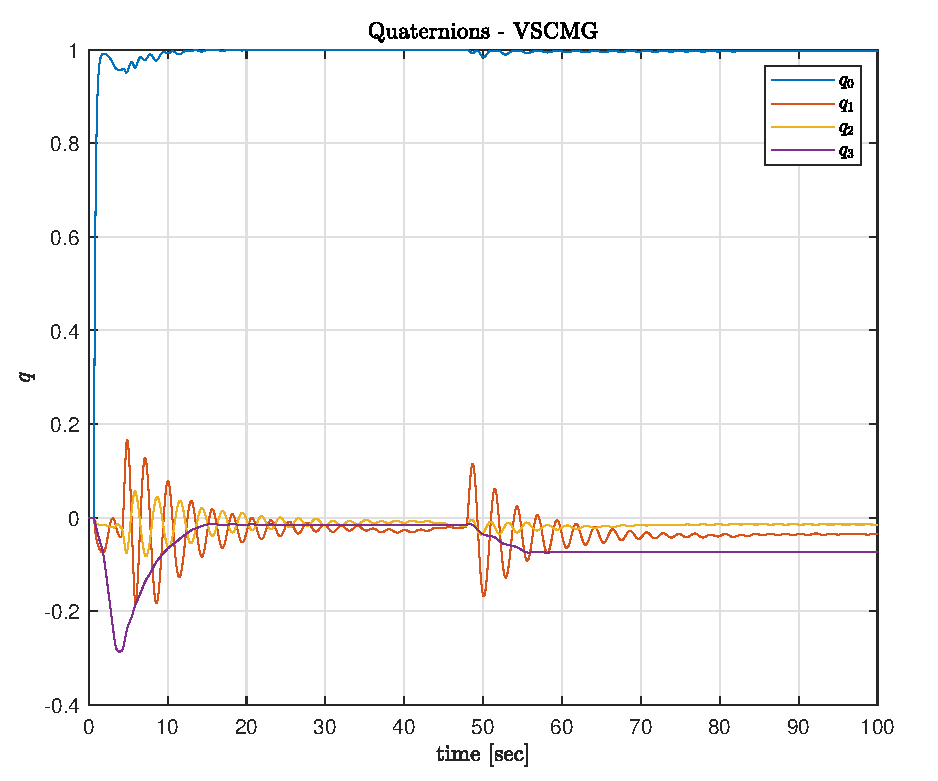
\includegraphics[width=1.0\textwidth]{figures/plots/exp/free-q1.pdf}
%    \caption{}
%    \label{fig:free-q1}
%\end{figure}

\begin{figure}[ht]
    \centering
    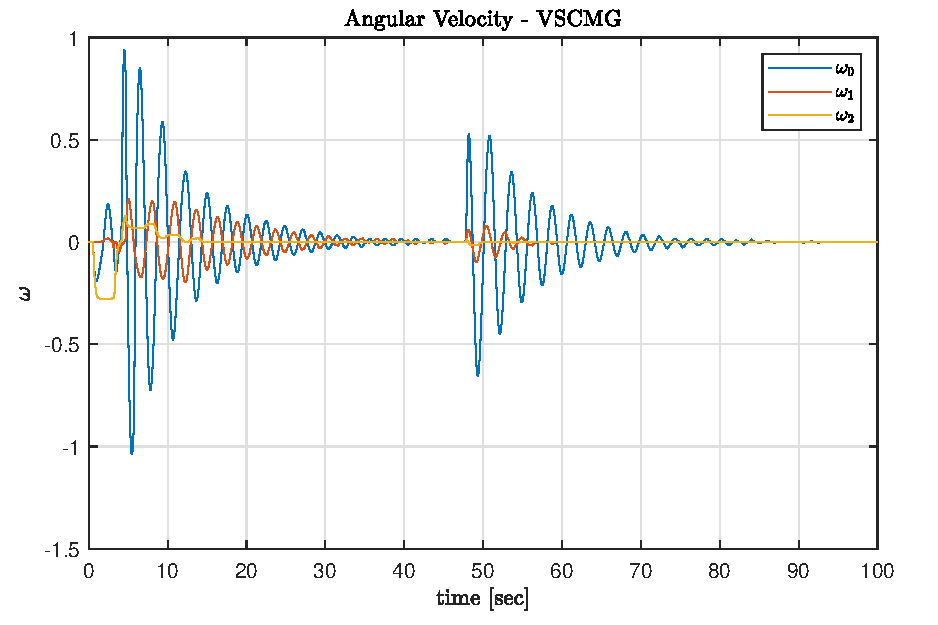
\includegraphics[width=0.7\textwidth]{figures/plots/exp/free-w1.pdf}
    \caption{ACS off free motion of test bed upon disturbance}
    \label{fig:free-w1}
\end{figure}

\begin{figure}[ht]
    \centering
    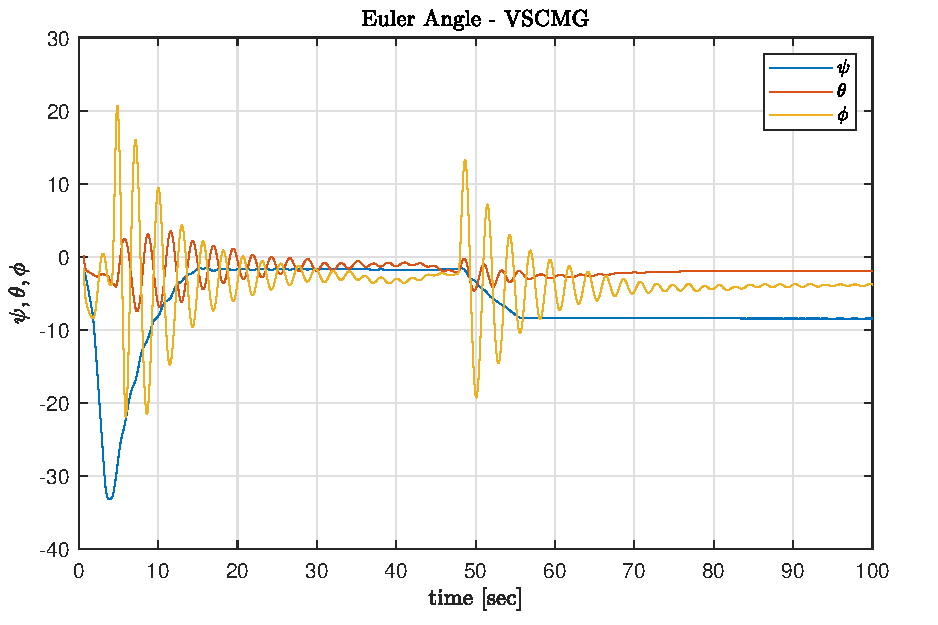
\includegraphics[width=0.7\textwidth]{figures/plots/exp/free-eul1.pdf}
    \caption{Free response of platform subjected to disturbance, Euler angles ($\deg$)}
    \label{fig:free-eul1}
\end{figure}

\section{Open Loop Control}
In order to test the command response of actuator and weather they are capable of overcoming the friction and are able to move platform is few open loop tests are conducted.
\subsection{Open Loop CMG}
As provision for producing gyroscopic torque, initially all the reaction wheels are accelerated to 3000 RPM with platform at rest and equal angular momentum of all RWs. All gimbal motors are commanded to rotate at 1 RPM angular velocity in order to produce torque along yaw axis. Initially at rest, platform start accelerating around yaw axis. as soon as gimbal angle crosses 180 degrees, net torque direction is reversed and platform starts de-accelerating first and later starts rotating in opposite direction. From \autoref{fig:cm-eul1} it is clear that maximum variation in attitude only around yaw axis and no significant change in roll and pitch is is visible. In \autoref{fig:cm-w1}, angular velocity along roll and pitch axis is osculating withing maximum amplitude of 0.2 rad/sec. Direction of angular velocity about yaw axis ($\omega_2$) does not change as rapidly as compared to roll and pitch axis, consequently making large deviation about yaw.

\begin{figure}
     \centering
     \begin{subfigure}[b]{0.45\textwidth}
     \centering
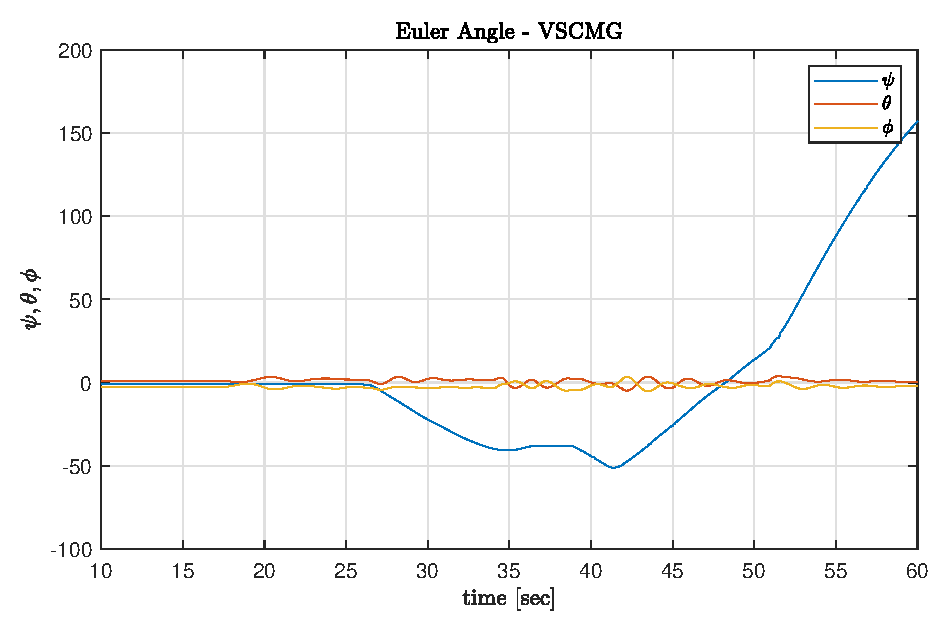
\includegraphics[width=1.0\textwidth]{figures/plots/exp/cm-eul1.pdf}
    \caption{Euler Angles ($\deg$)}
    \label{fig:cm-eul1}
    \end{subfigure}
     \begin{subfigure}[b]{0.45\textwidth}
     \centering
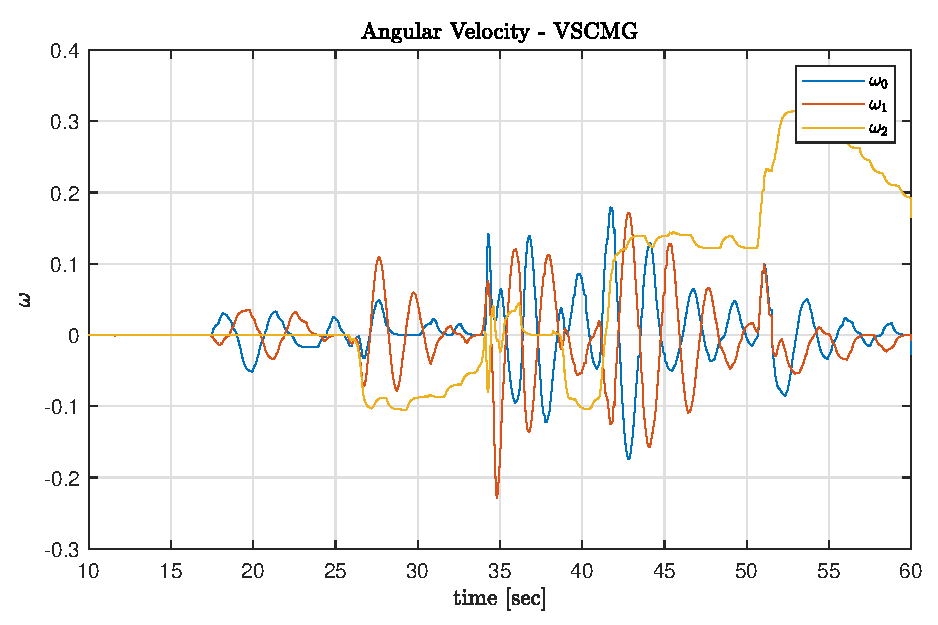
\includegraphics[width=1.0\textwidth]{figures/plots/exp/cm-w1.pdf}
    \caption{Body rates ($rad / \sec$)}
    \label{fig:cm-w1}

     \end{subfigure}
        \caption{Open loop maneuver results of CMG}
        \label{fig:ol.cmg}
\end{figure}


\section{Close Loop SR-VSCMG Control}
In this section results of VSCMG based steering law are presented considering only derivative feedback. Quaternion feedback gain $K_q$ is set to zero and angular velocity feedback gain $K_w = 0.6$ is selected after several iteration and testing. Initially platform is kept at res. All reaction wheels kept at zero RPM thus it is clear that CMG can not produce required torque. Close loop controller is turned on at 8 seconds and platform is manually disturbed by hand. From \autoref{fig:vs-w1} two disturbance events ca be clearly seen at 10 seconds and 15 seconds. For first disturbance, platform is tilted by hand. From first peak it is clear that only platform resist the tilt motion and angular velocities are damped within 3 seconds. Second disturbance seen at 15 seconds is small nudge to platform was compensated within 2 seconds with no steady state error beyond 5 seconds after disturbance event. 
\begin{figure}[ht]
    \centering
    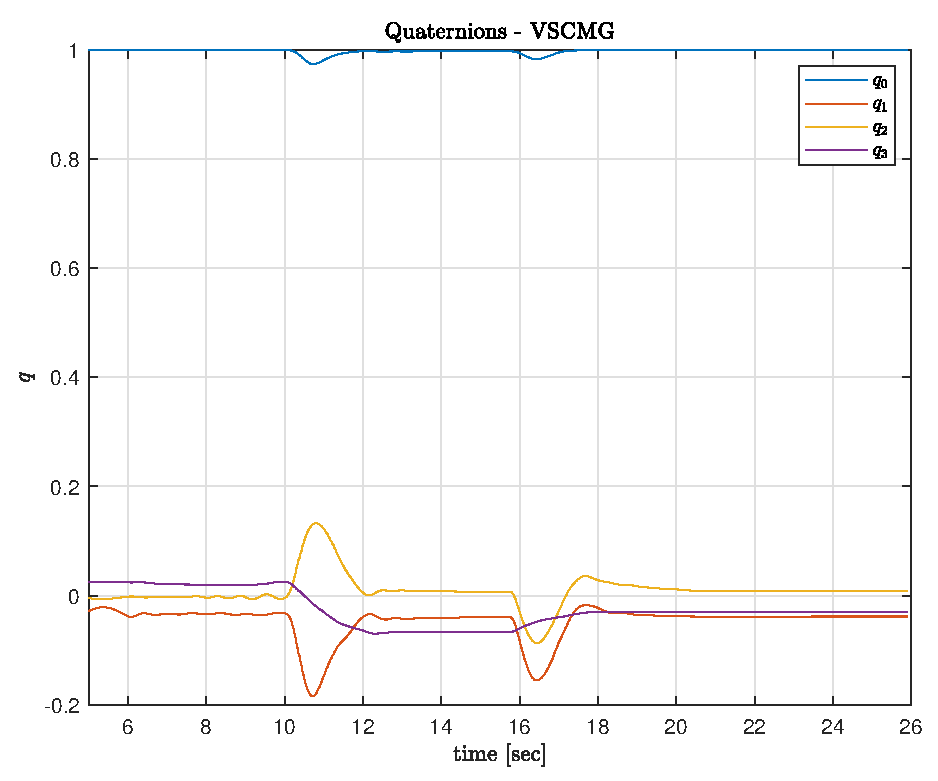
\includegraphics[width=0.7\textwidth]{figures/plots/exp/vs-q1.pdf}
    \caption{Close loop maneuver using VSCMG steering law with only derivative feedback - Platform quaternions}
    \label{fig:vs-q1}
\end{figure}
\begin{figure}[ht]
    \centering
    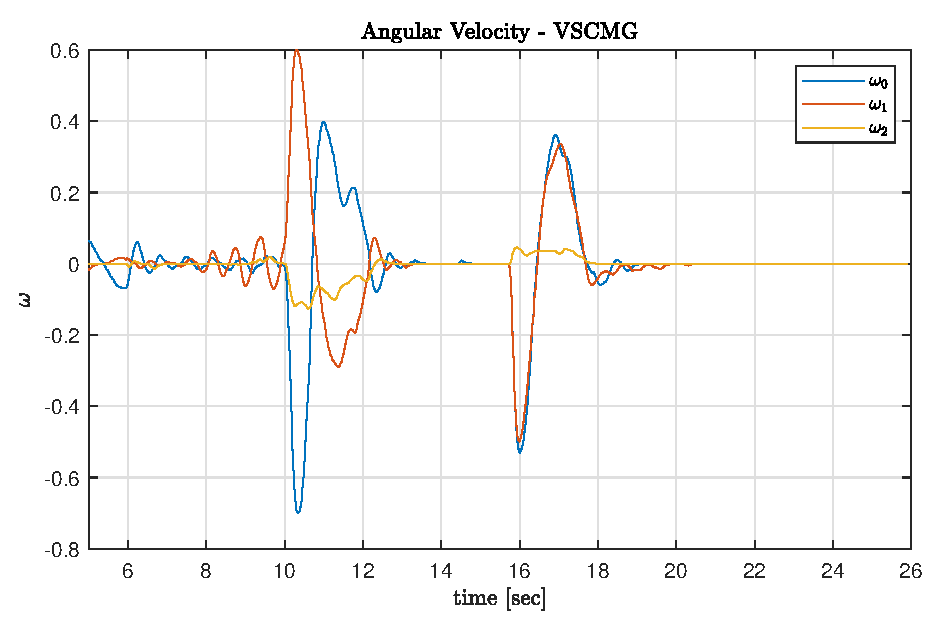
\includegraphics[width=0.7\textwidth]{figures/plots/exp/vs-w1.pdf}
    \caption{Close loop maneuver using VSCMG steering law with only derivative feedback - Platform angular velocities ($rad / \sec$)}
    \label{fig:vs-w1}
\end{figure}
Only reaction wheel based controller was sufficient to counteract the external disturbances. Euler angles shown in \autoref{fig:vs-eul1} are computed from quaternions. It is clear that although platform was balanced to maintained at the level, offset in roll and pitch are visible because of uncertainty in placement of IMU which is at  offset from platform which introduce orientation error. Despite these uncertainties due to placement of IMU, controller is able to counteract the disturbance and quickly bring platform to steady state.
\begin{figure}[ht]
    \centering
    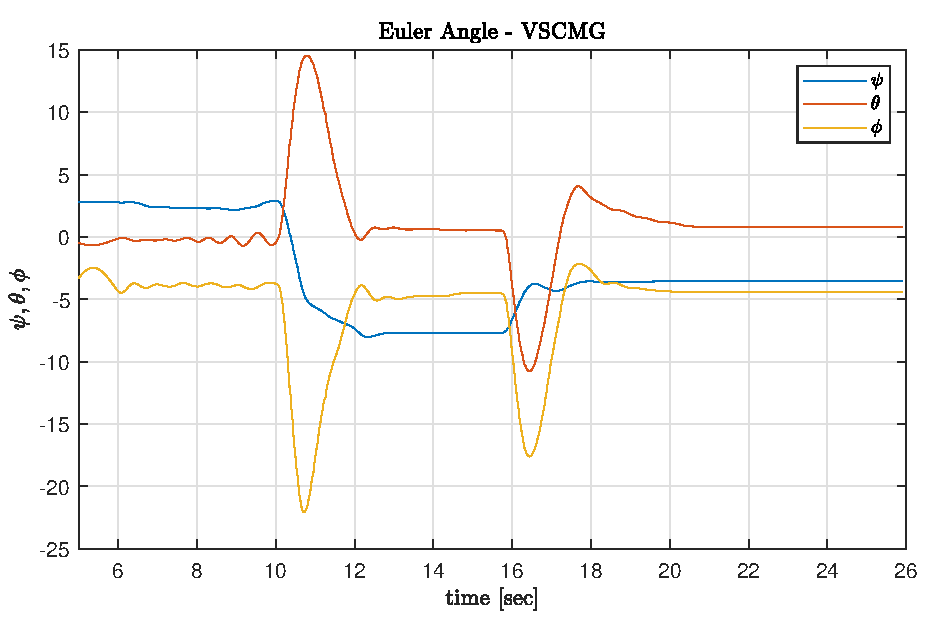
\includegraphics[width=0.7\textwidth]{figures/plots/exp/vs-eul1.pdf}
    \caption{Close loop maneuver using VSCMG steering law with only derivative feedback - Euler angles ($\deg$)}
    \label{fig:vs-eul1}
\end{figure}

After several iterations of testing, many problems were analyzed of which most important is very small oscillations persist which were not visible in each test with same input parameters. Controller has different steady state performance for and long time is needed to compensate disturbances, this was due to lower battery voltage and can be solved by keeping batteries above minimum threshold or by updating controller gain based on available power. Orientation uncertainties can be removed by recording IMU offset and introducing offset rotation matrix. Gimbal angle is measured through magnetic encoder which provide absolute angular feedback but are not linear due to offset in sensor and shaft magnet. Since steeper motors are used for gimbal, Encoder error can be compensated by keeping track of motor steps and updating the zero position every time magnet crosses the zero position. Thus magnetic encoders will be only used as reference. Breathless motors used for reaction wheels are driven using back EMF feed back based motor controller. These type of controllers are not capable of running motors at lower speed and significant dead band is present near zero RPM, this is introduces jerks at lower speeds. Hall sensor based controllers can be used to have better control at lower speed. Hall sensor based controllers keeps track of rotor orientation and activate coils in sequence based on pre determined lookup table.
\\
\\
Photos of custom-built test setup for VSCMG is shown in \autoref{fig:tv-tb-stand} to \autoref{fig:sv-tb}. Small 3D printed tripod with a metal coin at the top along side complete VSCMG platform is shown in \autoref{fig:tv-tb-stand}. \autoref{fig:tv-tb} and \autoref{fig:sv-tb} are top and side view of complete test setup.

\begin{figure}
    \centering
    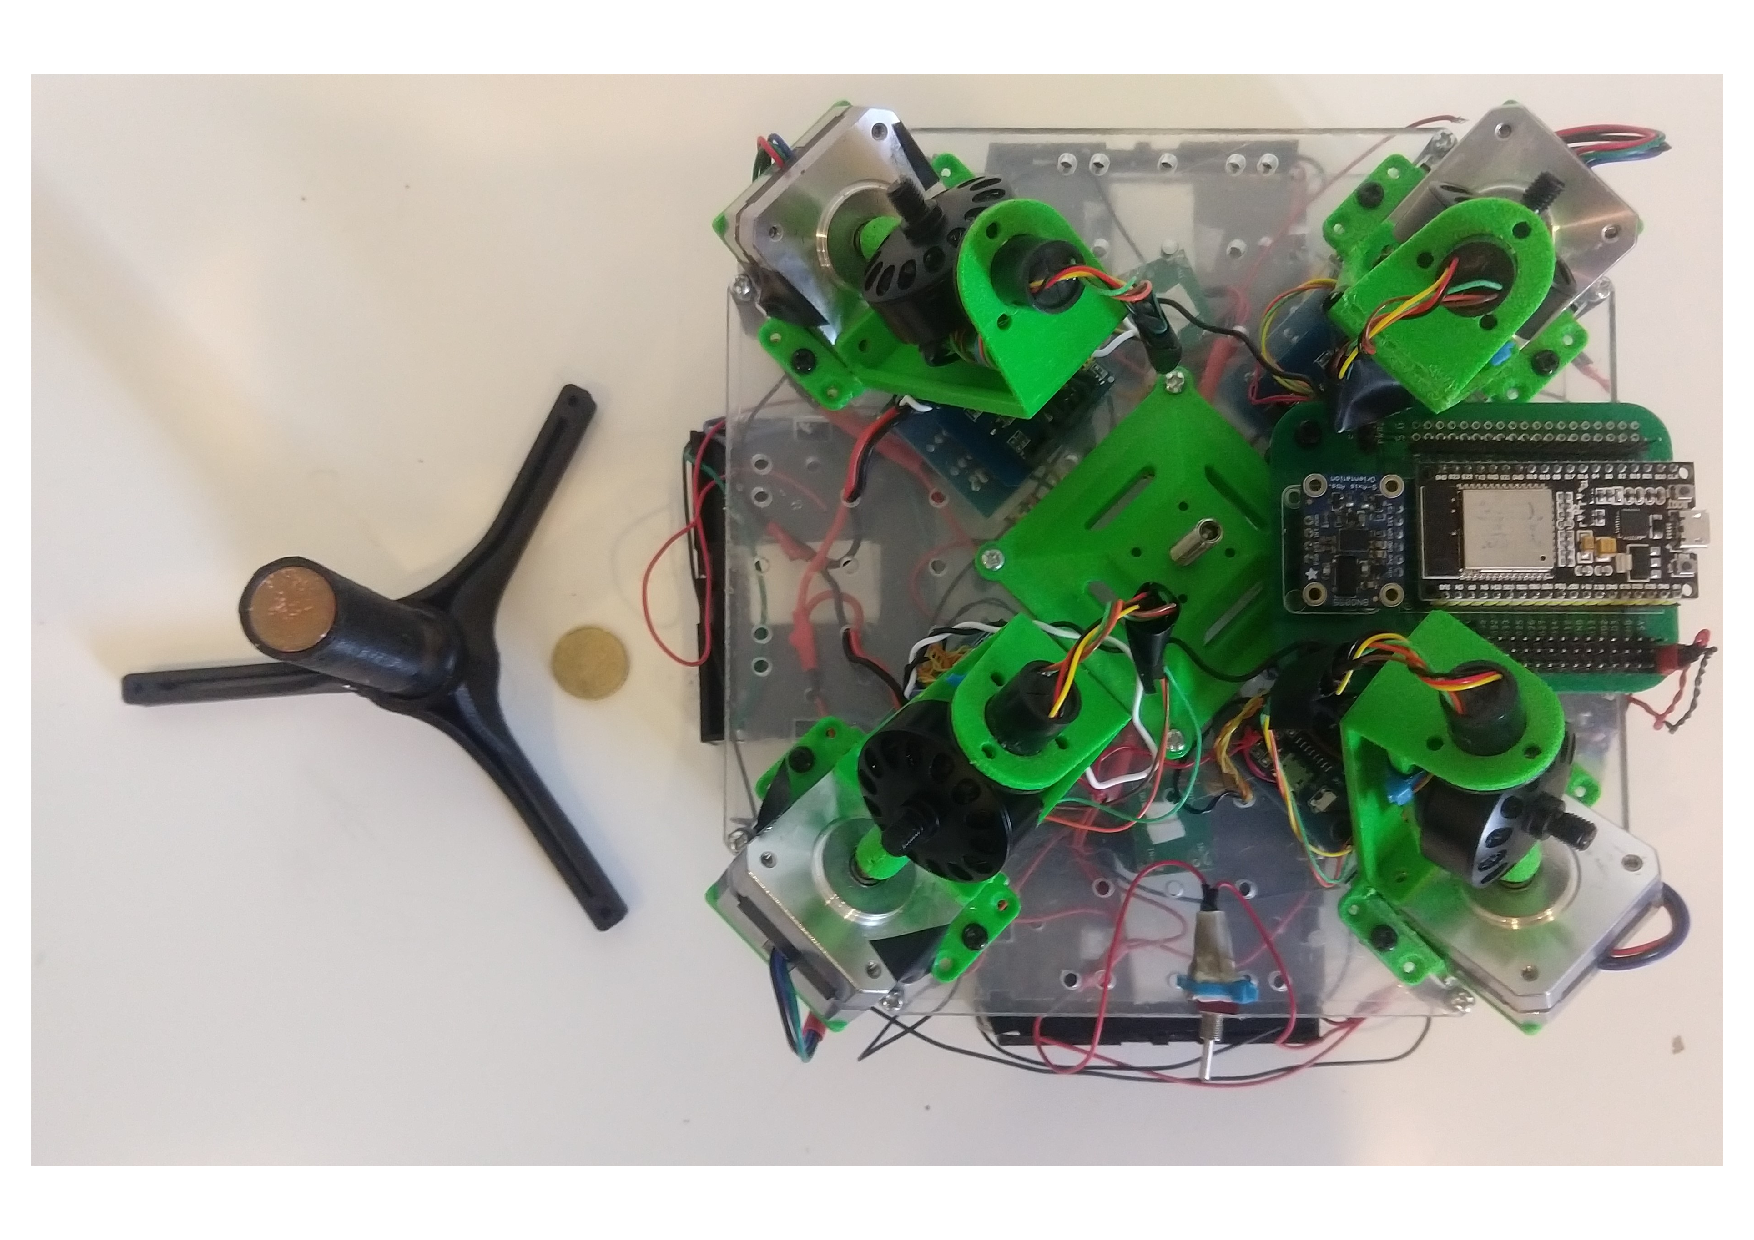
\includegraphics[width=\textwidth]{figures/photos/tb-stand-tv.pdf}
    \caption{Top view of custom-built VSCMG experimental test bed and tripod}
    \label{fig:tv-tb-stand}
\end{figure}

\begin{figure}
    \centering
    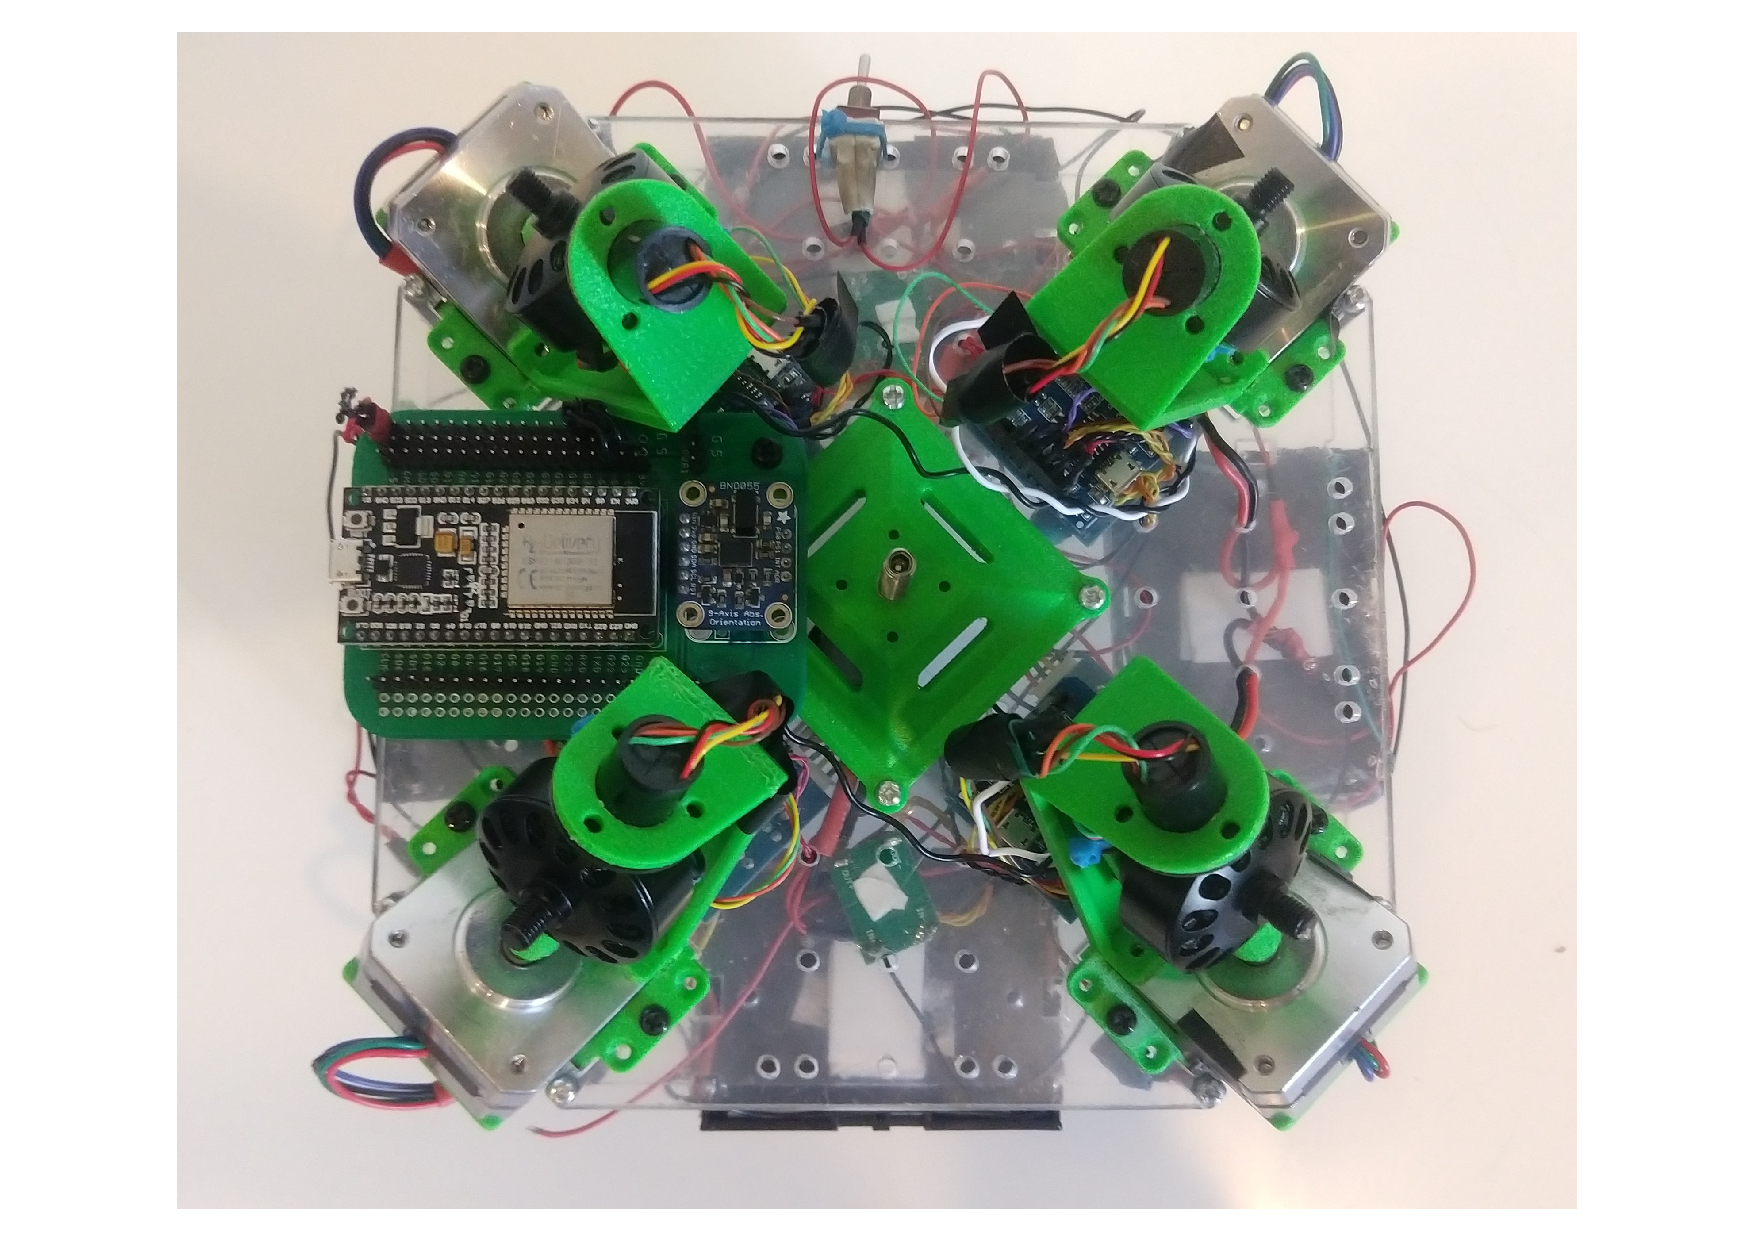
\includegraphics[width=\textwidth]{figures/photos/tv-tb.pdf}
    \caption{Top view of custom-built VSCMG experimental test bed balancing on tripod}
    \label{fig:tv-tb}
\end{figure}

\begin{figure}
    \centering
    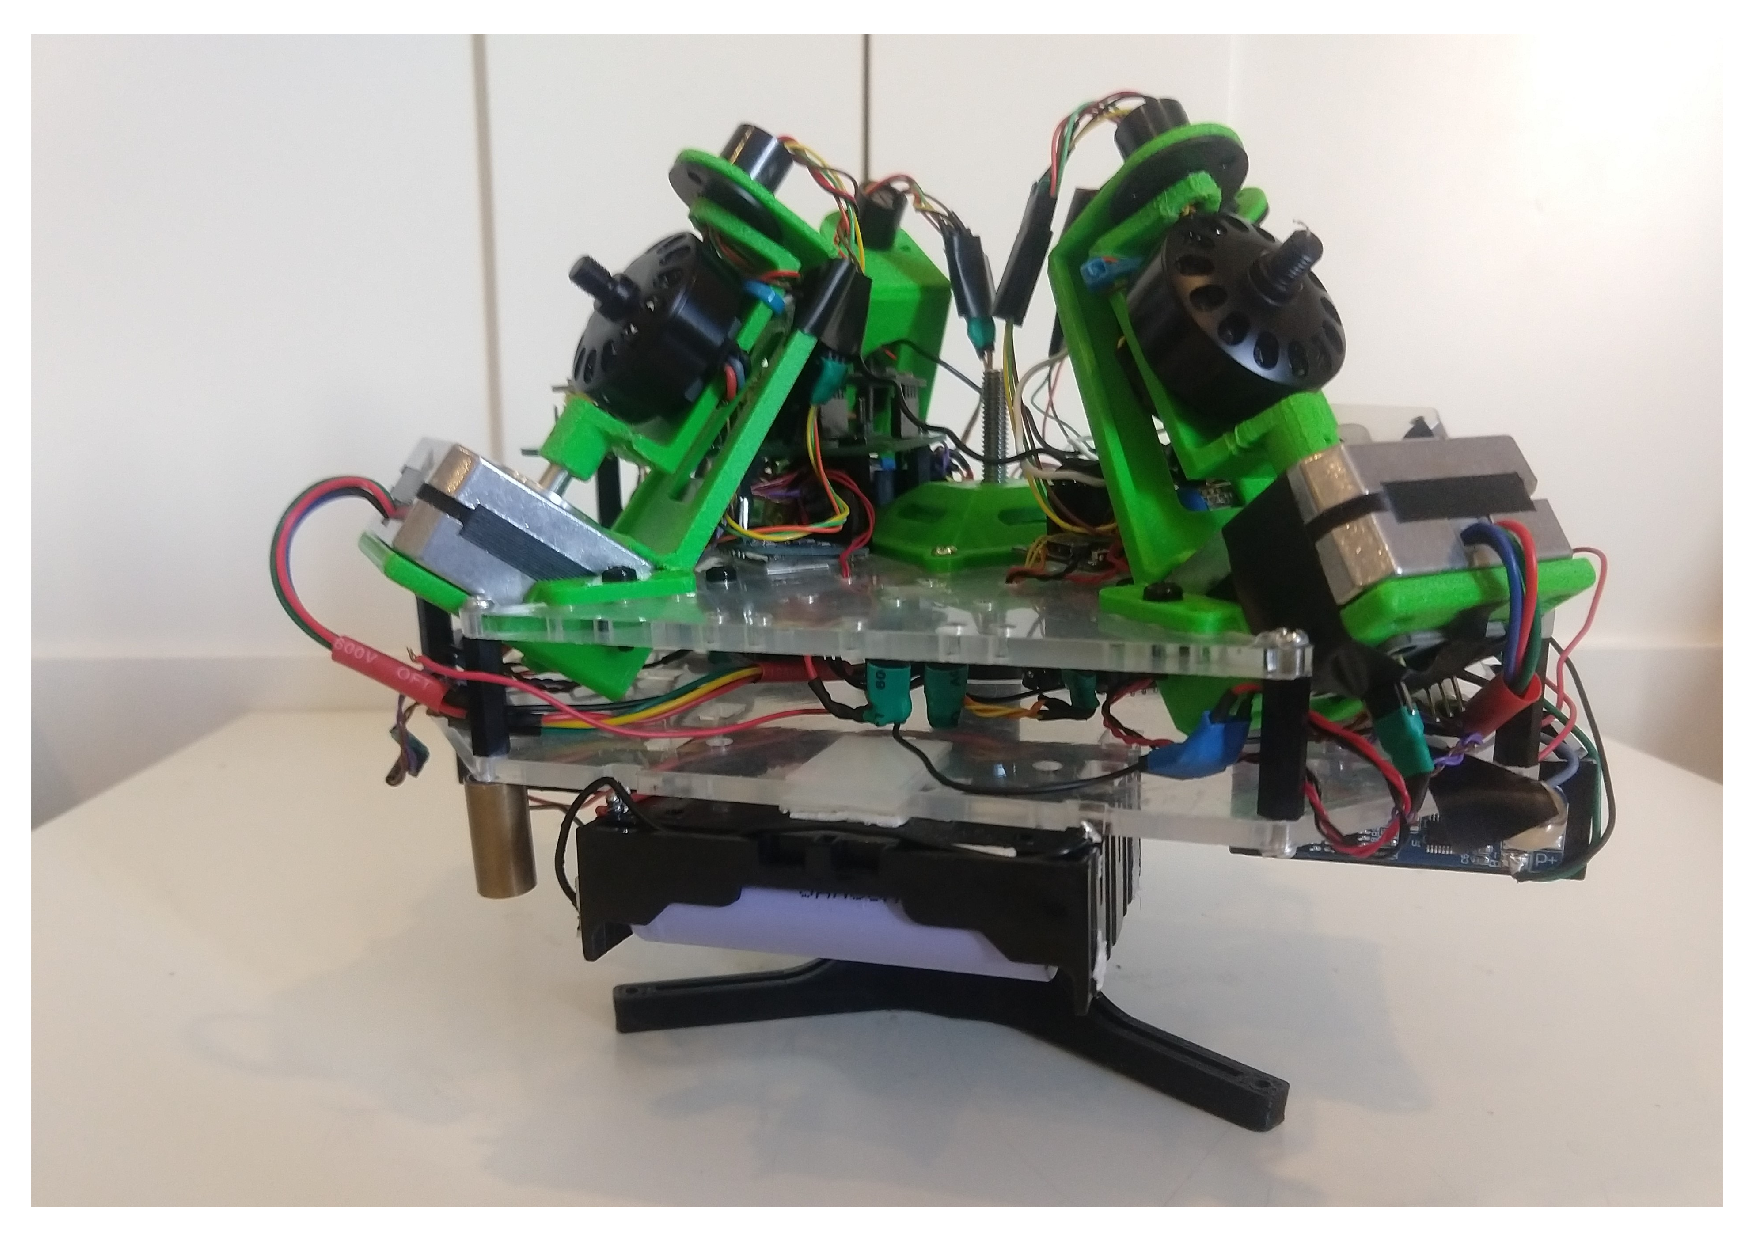
\includegraphics[width=\textwidth]{figures/photos/sv-tb.pdf}
    \caption{Side view of custom-built VSCMG experimental test bed balancing on tripod}
    \label{fig:sv-tb}
\end{figure}
